\documentclass[authoryear, 12pt,5p, Times]{elsarticle}
\usepackage[hypcap]{caption}
\usepackage{float}
\usepackage[hidelinks]{hyperref} 
 \usepackage{gensymb}
\usepackage{subcaption}
\usepackage{url}
%\renewcommand\thefootnote{\fnsymbol{\dagger}}
\usepackage[symbol*]{footmisc}
\begin{document}
%\footnote{This is a footnote}
\begin{frontmatter}
\title{Photon Counting \& the Statistics of Light}
\author{\today \\ \quad \\Jung Lin (Doris) Lee\\ dorislee@berkeley.edu\\Group partners: Jennifer Ito, Manuel Silvia\\Prof. James Graham, UGSI Heechan Yuk, Isaac Domagalski}
	\begin{abstract}
    %key objective, method, principle conclusion 
	 We present the methods used to conduct the photon counting experiment and the statistical results obtained from the collected data. By varying the brightness of the light source, we found that photon arrival rate increases, as seen from the decreased number of events .(\textbf{modify this??})Analysis on a single data set shows that as the the number of events in an experiment increases, the sample mean($\bar{x}$) converges to the theoretical mean($\mu$). However since systematic effects can not be eliminated by increasing number of events, we mitigate the effect of afterpulsing by vetoing photon arrival events that occurred immediately after another. The processed data results in a histogram that align very closely to exponential distribution. In addition, binned data for a fixed time interval also matches closely with the Poisson distribution. Therefore, by fitting the distribution we obtain the sample mean parameter of the experiment.  
	\end{abstract}
\end{frontmatter}
\section{Introduction\label{intro}}
\indent Photon statistics are the fundamental basis to optical astronomy since they constitute the data we collect in optical astronomy. 
are important to astronomy because 
optical astronomy 
can be used to study galaxy morphology, individsual sources or conduct statistical studies for cosmomlgogical studies.
Large sky surveys such as the Sloan Digital Sky Survey(SDSS; York et al.) and the Dark Energy Survey (DES; The Dark Energy Collaboration) imaging data in the optical wavelength.
\indent In this experiment, we recorded the arrival of photons from an LED and analyze
 In section 2, I will describe the experimental method that my group used to take the data and the results that we obtained. Subsequently, section 3 introduces the various statistical measures that we can use to describe the findings and observation on  a single dataset, including the effect of binning the data into histograms. Section 4 describes the two probability density functions that are relevant to these histograms and dataset.
\section{Experiments\label{experiment}}
	\subsection{Methods}
\indent The arrival of a photon is registered by the photomultiplier tube (PMT), and data was acquired using the CoinPro software. The resulting processed data file is a series of time stamps of when the data arrived. Since CoinPro is ran on a 32-bit machine, we can see the cycling through of time in FIG REF. Although absolute time stamp is the recorded quantity, it is often more useful to consider the time elapsed between two consecutive events ($\texttt{dt}$) as plotted in Fig. in order to get a sense of  the photon arrival rate for some sample waiting time.
\begin{figure}[h]
\centering
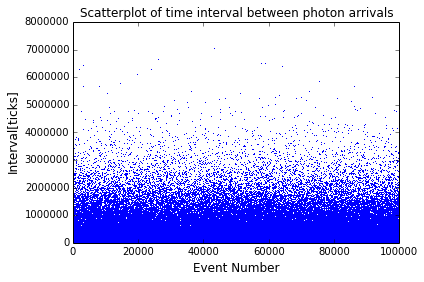
\includegraphics[width=0.5\textwidth]{figures/interval_scatterplot}
\caption{With the removal of after pulse event, we can see that there is a decline in the number of events. This makes sense because we are doing an interval cut at 3000 clock ticks, which should result in a clear boundary at y=3000 but this can not be seen due to the large range of interval value that the y-axis spans over. The data representation in Fig.\ref{changeLED} and \ref{fitted_histo_gate_or_no} better shows the the effect of gating afterpulses. }
\label{scatterplot}
\end{figure}
\\
\indent Sometimes noise pulses resembling Fig.\ref{afterpulse} can be observed after the original pulse. These events are caused by  the ionization of residual gas molecules in the PMT's vacuum chamber.  We eliminate this systematic effects by cutting away data with subsequent pulses lie within the time frame of 2.5$\mu$s  after an original pulse as shown in Fig.\ref{fitted_histo_gate_or_no}.

\begin{figure}[h]
\centering
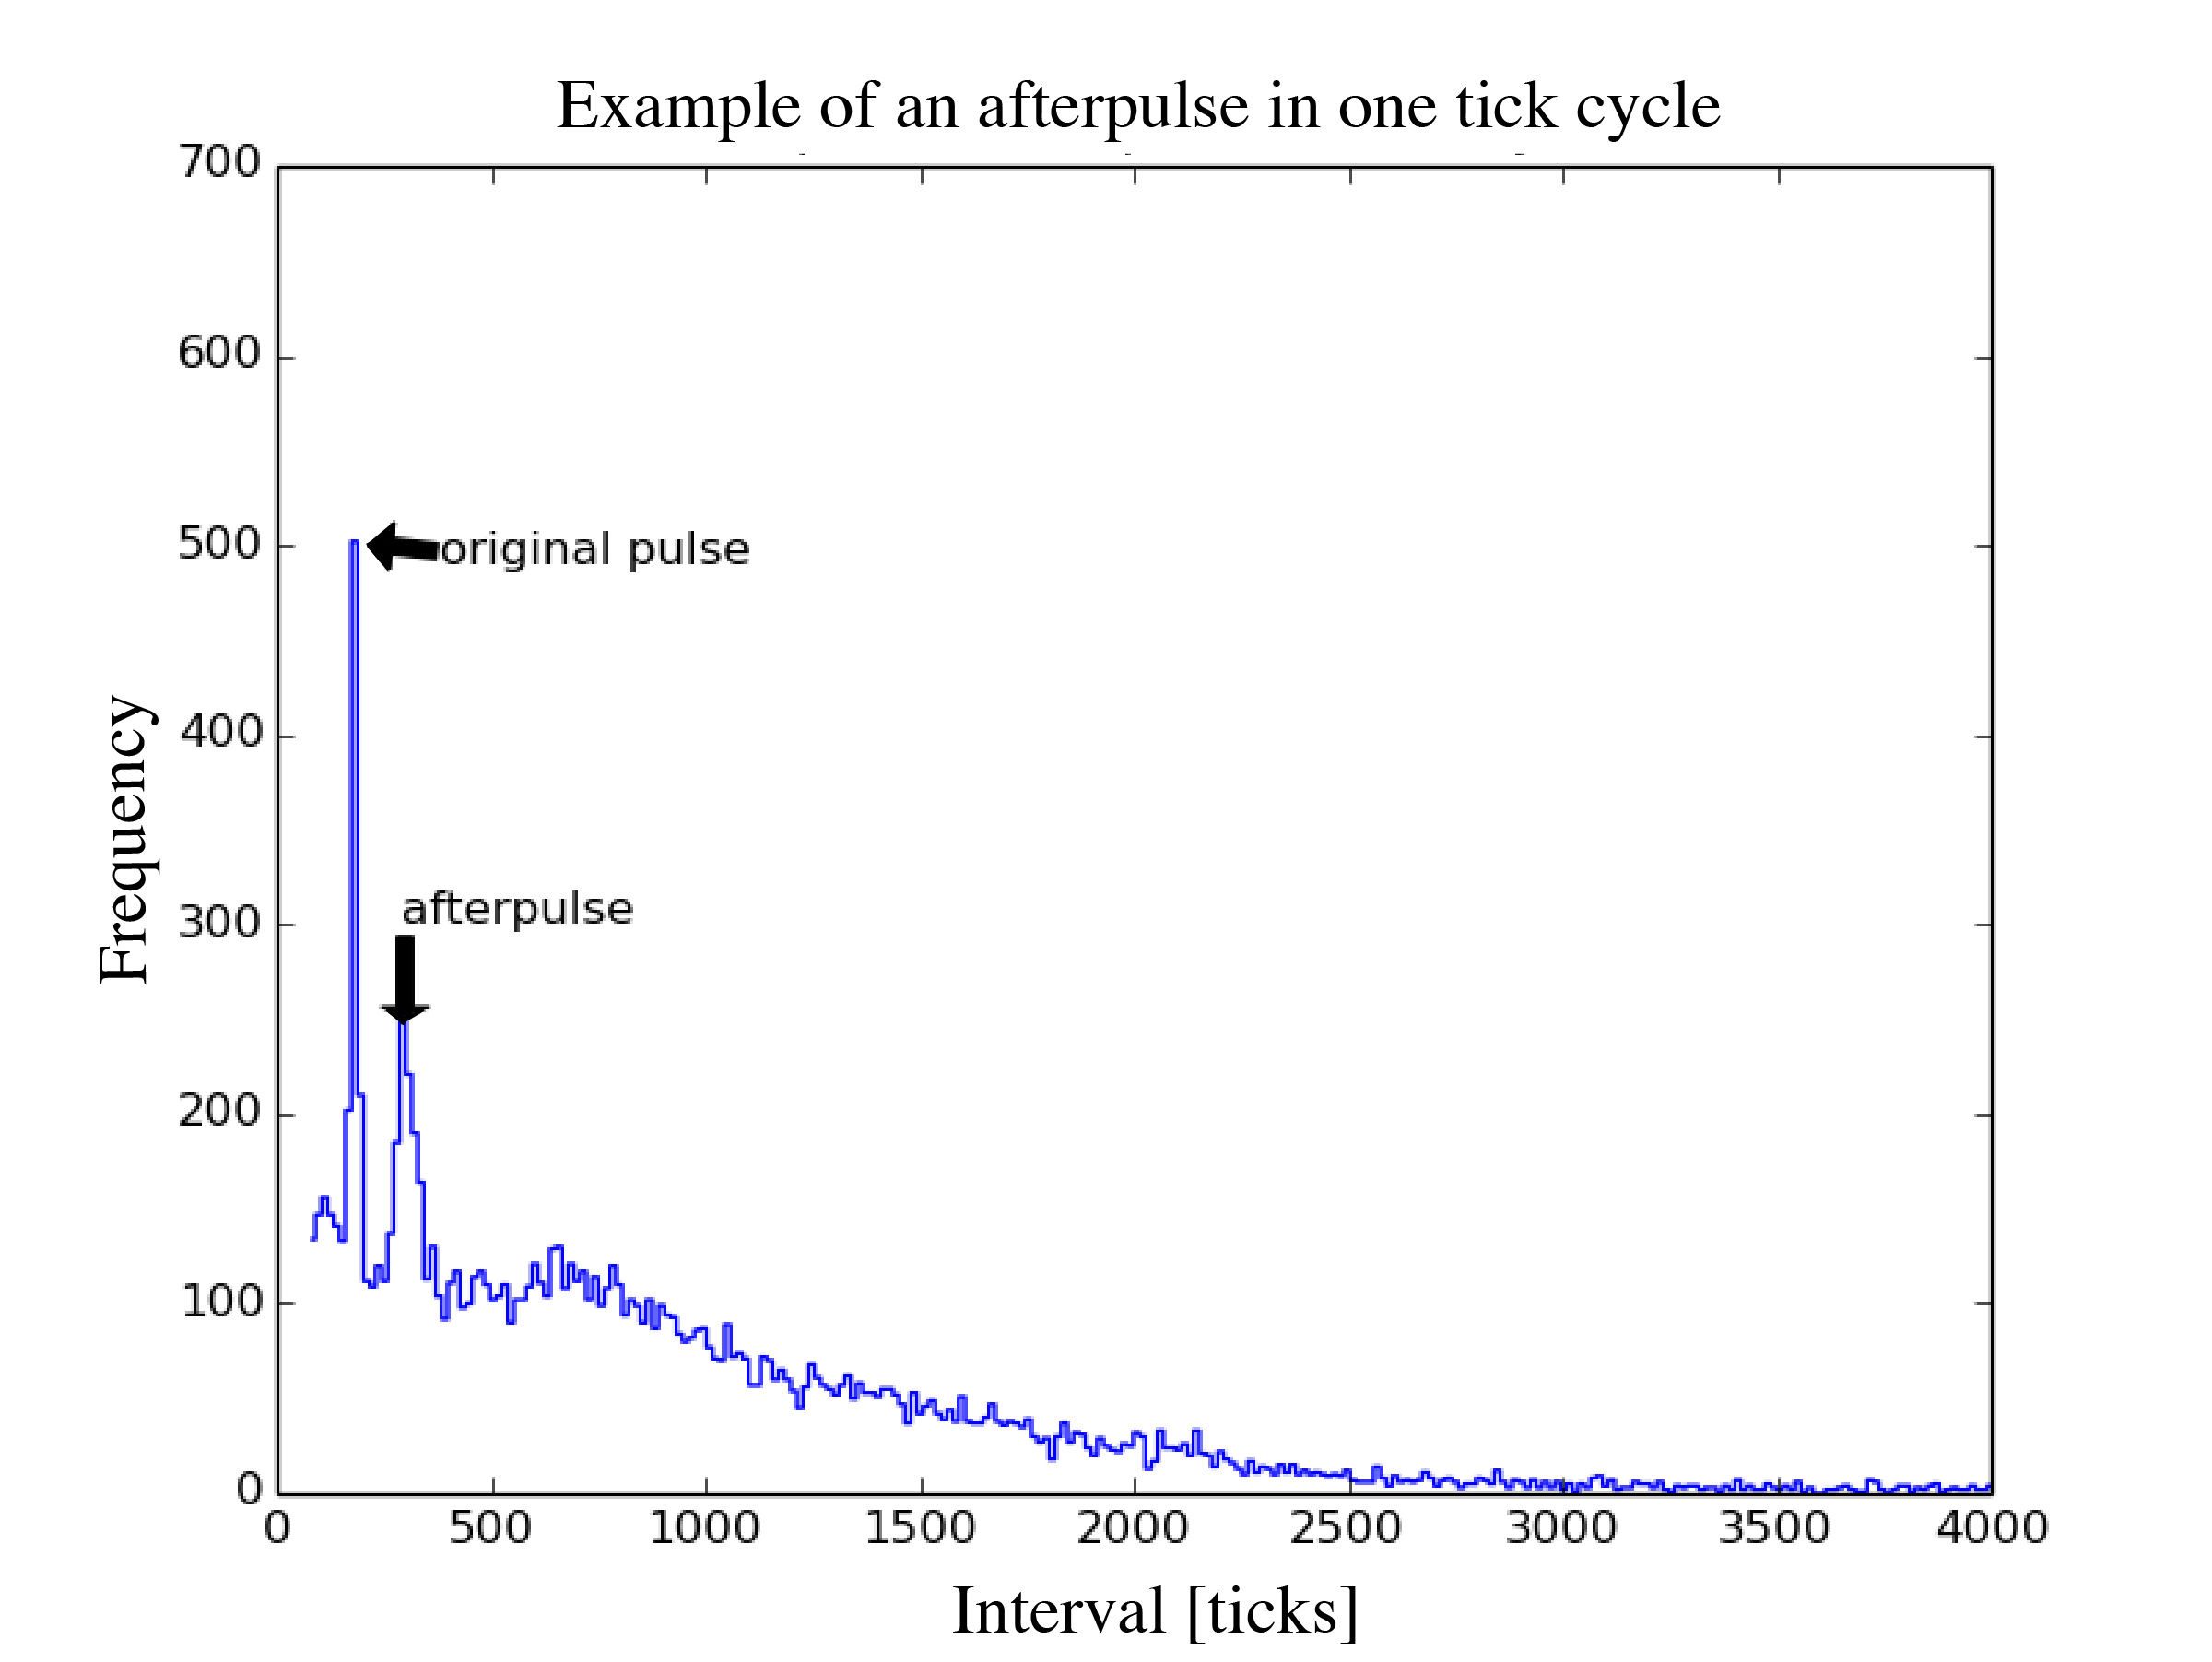
\includegraphics[width=0.5\textwidth]{figures/afterpulse}
\caption{With a histogram of bin size = 500,000, the two peaks (original and afterpulse) as well as a gradual decline of ticks in the next 3000 clock ticks can be seen here.}
\label{afterpulse}
\end{figure}
   \subsection{Changing LED Brightness\label{changeLEDbrightness}}
\indent By listening to ticks on the squawker, there was no detectable difference from the 3 o'clock off position to the 12 o'clock position. Therefore, we started off at the 12 o'clock location and went to the max location ($\approx$90\degree), diving this region into 6 equal parts \footnote{Although it seems like only 5 data points are shown in the plot, this is merely an artifact of the choice of data representation as circles as  the first two data points lie so closely that they are almost indistinguishable. This is easily verified by using the dot representation with \texttt{matplotlib's} `,`setting} is roughly 18\degree  increments. Even though the measurement of the LED brightness is eyeballed and not that precise, it did not significantly affect the plot since the the data point should fall on the $\sigma=\bar{x}$ line since the $\sigma$ and $\mu$ of an exponential distribution is always equal.
\begin{table}
    \center
    \begin{tabular}{l|l}
    Intensity[\degree] & Final time stamp in time series [ticks] \\ \hline
    0                                    & 86447071309                                     \\
    18                                   & 68475846523                                     \\
    36                                   & 35127973096                                     \\
    54                                   & 7517634481                                      \\
    72                                   & 5787954870                                      \\
    90 (max)                             & 5558407093                                      \\
    \end{tabular}
    \caption{Intensity is specified as the LED control knob position in degrees, as described earlier in Sec.\ref{changeLEDbrightness}. Since we are taking a fixed number of photon arrival events, as the brightness increases, the faster photon arrival rate means that 10,000 event count finishes faster than it did for lower brightness; thus, accounting for the smaller time stamp values.}
\end{table}
\begin{figure}[h]
%Last timestamp in the reconstructed time series
\centering
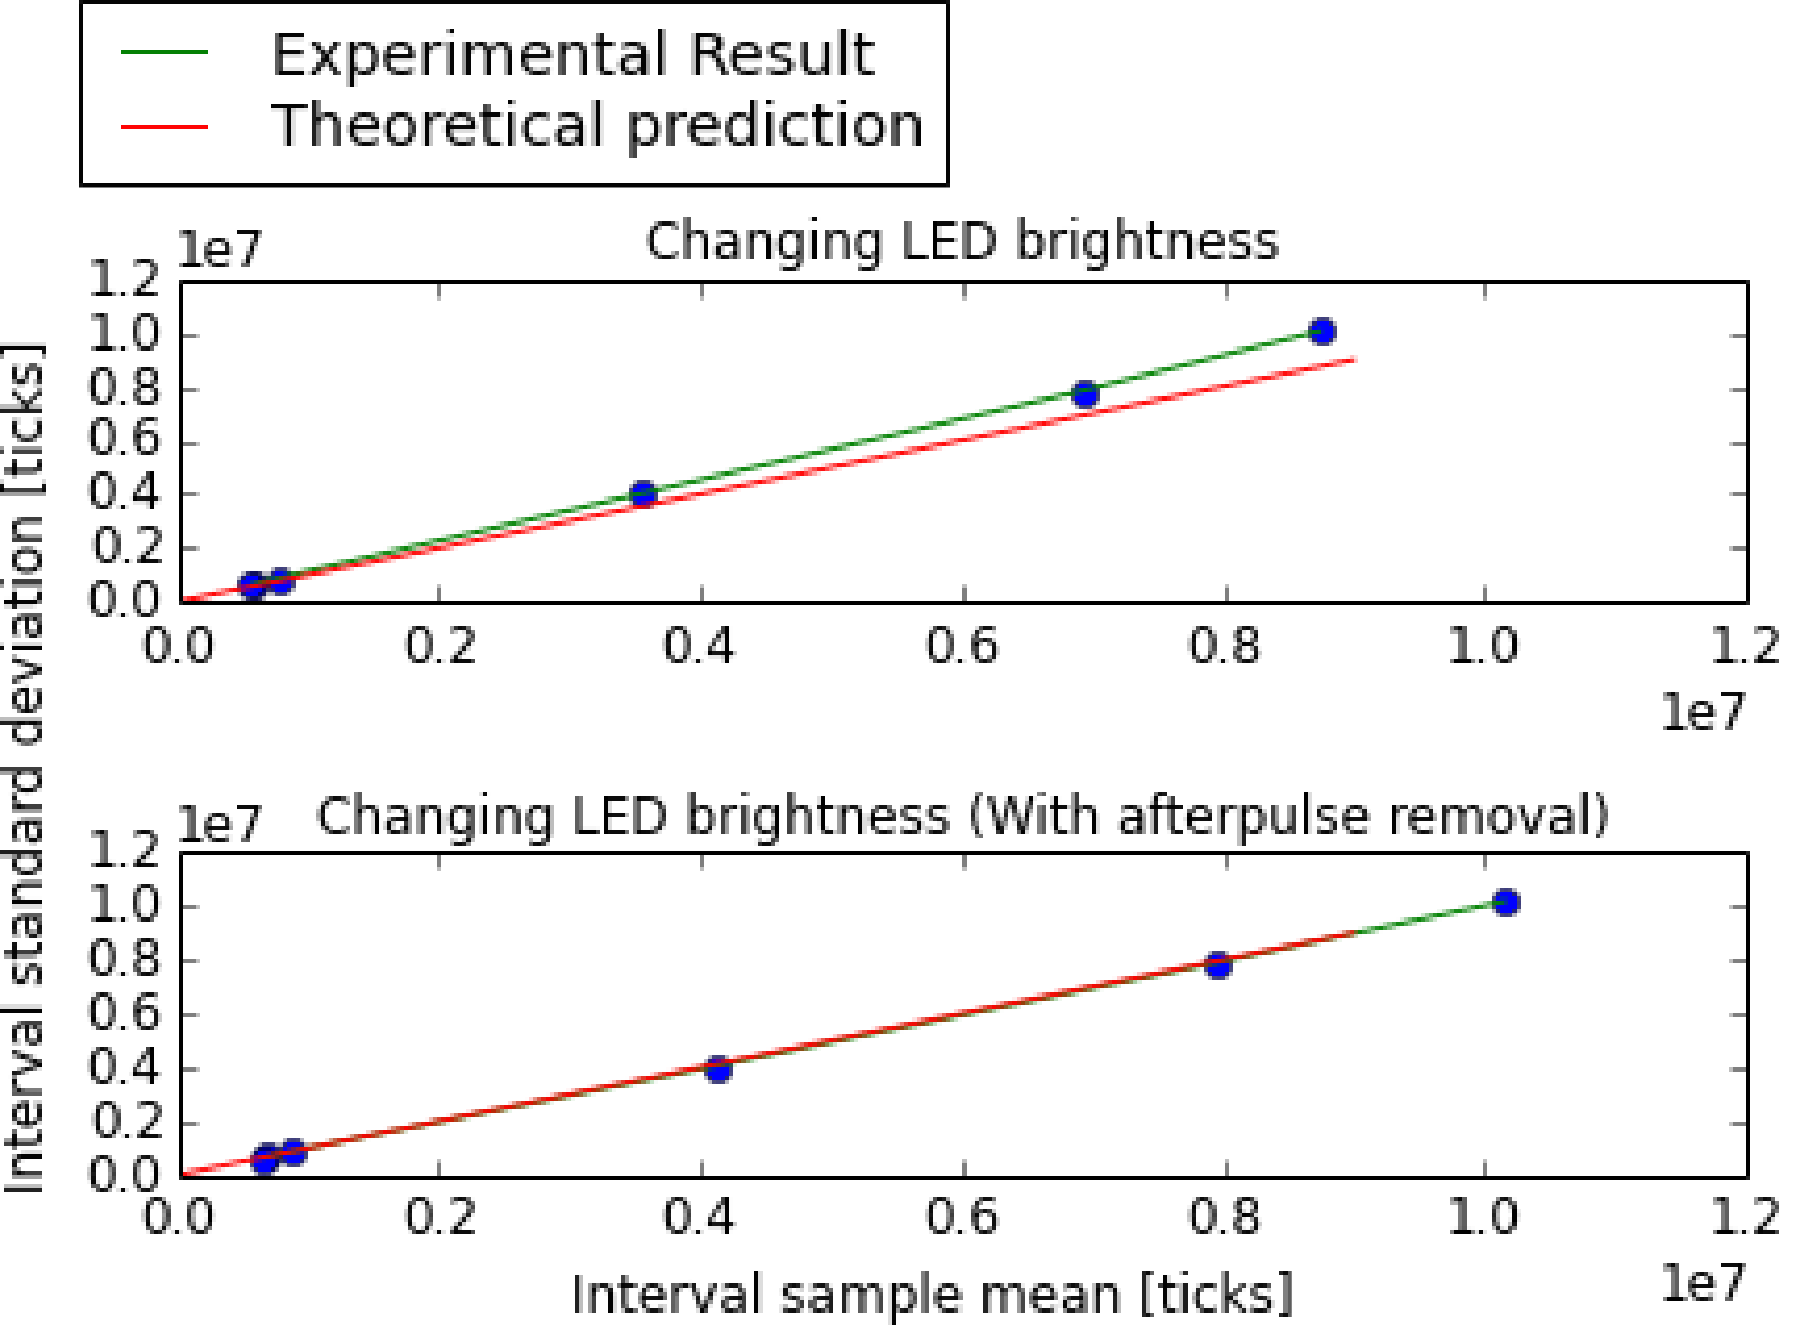
\includegraphics[width=0.5\textwidth]{figures/changeLED}
%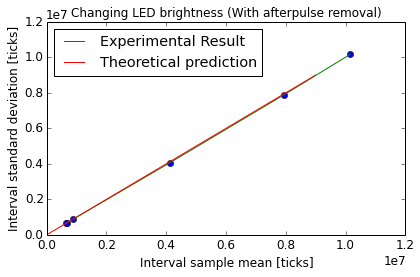
\includegraphics[width=0.5\textwidth]{figures/changeLED_gating}
\caption{The slope of the line should be one since both the standard deviation and the sample mean of each dataset is equal to the single-parameter $\tau$ in the exponential distribution. We find that gating the afterpulses causes the $\bar{x}$ to get closer to $\mu$. }
\label{changeLED}
\end{figure}
\section{Descriptive Statistics and Histograms\label{stats}}
Using the N=100,000 dataset with LED on the maximum brightness setting, we obtain a sample mean of 561571.83 and the standard deviation is  637988.76 on the whole dataset of 99833 events \footnote{CoinPro does not stop the event count at exactly 100,000 events.}. This is the most precise measure of the statistical quantity for the data collected since the more data that we consider when computing these quantitative , the closer the sample mean converges to the mean value as shown in Fig. \ref{stat_converging}. Higher precision measurement of $\bar{x} $ and $\sigma$ can be obtained by taking a sample of larger N so that $\bar{x} \rightarrow \mu$, but this does not ameliorate any systematic effect such as dark current or afterpulses.
 	\begin{figure}[h]
		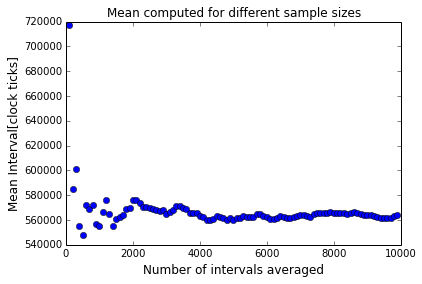
\includegraphics[width=0.5\textwidth]{figures/converging_mean}
		\caption{Large fluctuation in computed mean decreases as we use larger datasets to compute the mean value.}
		\label{stat_converging}
	\end{figure}
	\subsection{Standard Deviation of the Mean (SDOM)}
	 	\begin{figure}[h]
		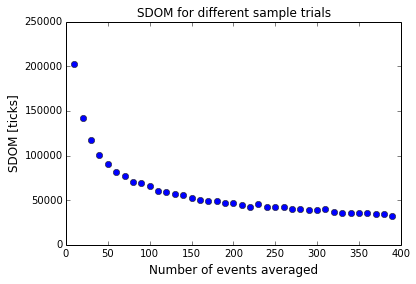
\includegraphics[width=0.5\textwidth]{figures/sdom_exp_graph}
		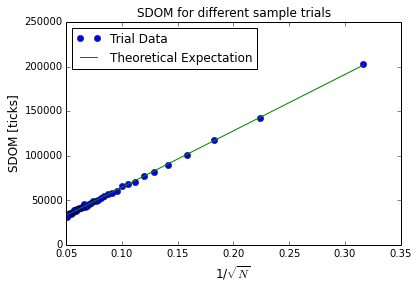
\includegraphics[width=0.5\textwidth]{figures/sdom_linear}
		\caption{SDOM}
		\label{stat_converging}
	\end{figure}
\section{Photon Statistics\label{pstats}}
	
 	\subsection{Exponential Distribution}
 	Exponential distribution described by Eq.\ref{exp_distr} governs the histogram of $\texttt{dt}$, the elapsed time between photon arrival event.
\begin{equation} \label{exp_distr}
 P(t,\tau)=\frac{1}{\tau}e^{-\frac{t}{\tau}}
\end{equation}
 	 A defining characteristic of the exponential distribution is that it is continous``memorylessness``. In this case, the photon arrival rate at some moment in time,t, is not dependent on the photon arrival rate prior to time t.  The green curve in Fig.\ref{fitted_histo_gate_or_no} is the plotted from the analytical solution shown in Eq.\ref{int_exp}, which is obtained from integrating the exponential distribution with a step-size $\Delta t =1.42x10^7$and  $\tau$ set as the mean of the $\texttt{dt}$ dataset .  
 	 \begin{equation}\label{int_exp}
 	 \int^{t+\Delta t}_\tau\frac{1}{\tau}e^\frac{t}{\tau}dt=-e^\frac{t+\Delta t}{\tau}+e^\frac{t}{\tau}
	\end{equation} 	  
Since the exponential probability density function (PDF) is normalized to one, this result is scaled by the number of events to fit the histogram.
 	\begin{figure}[h]
		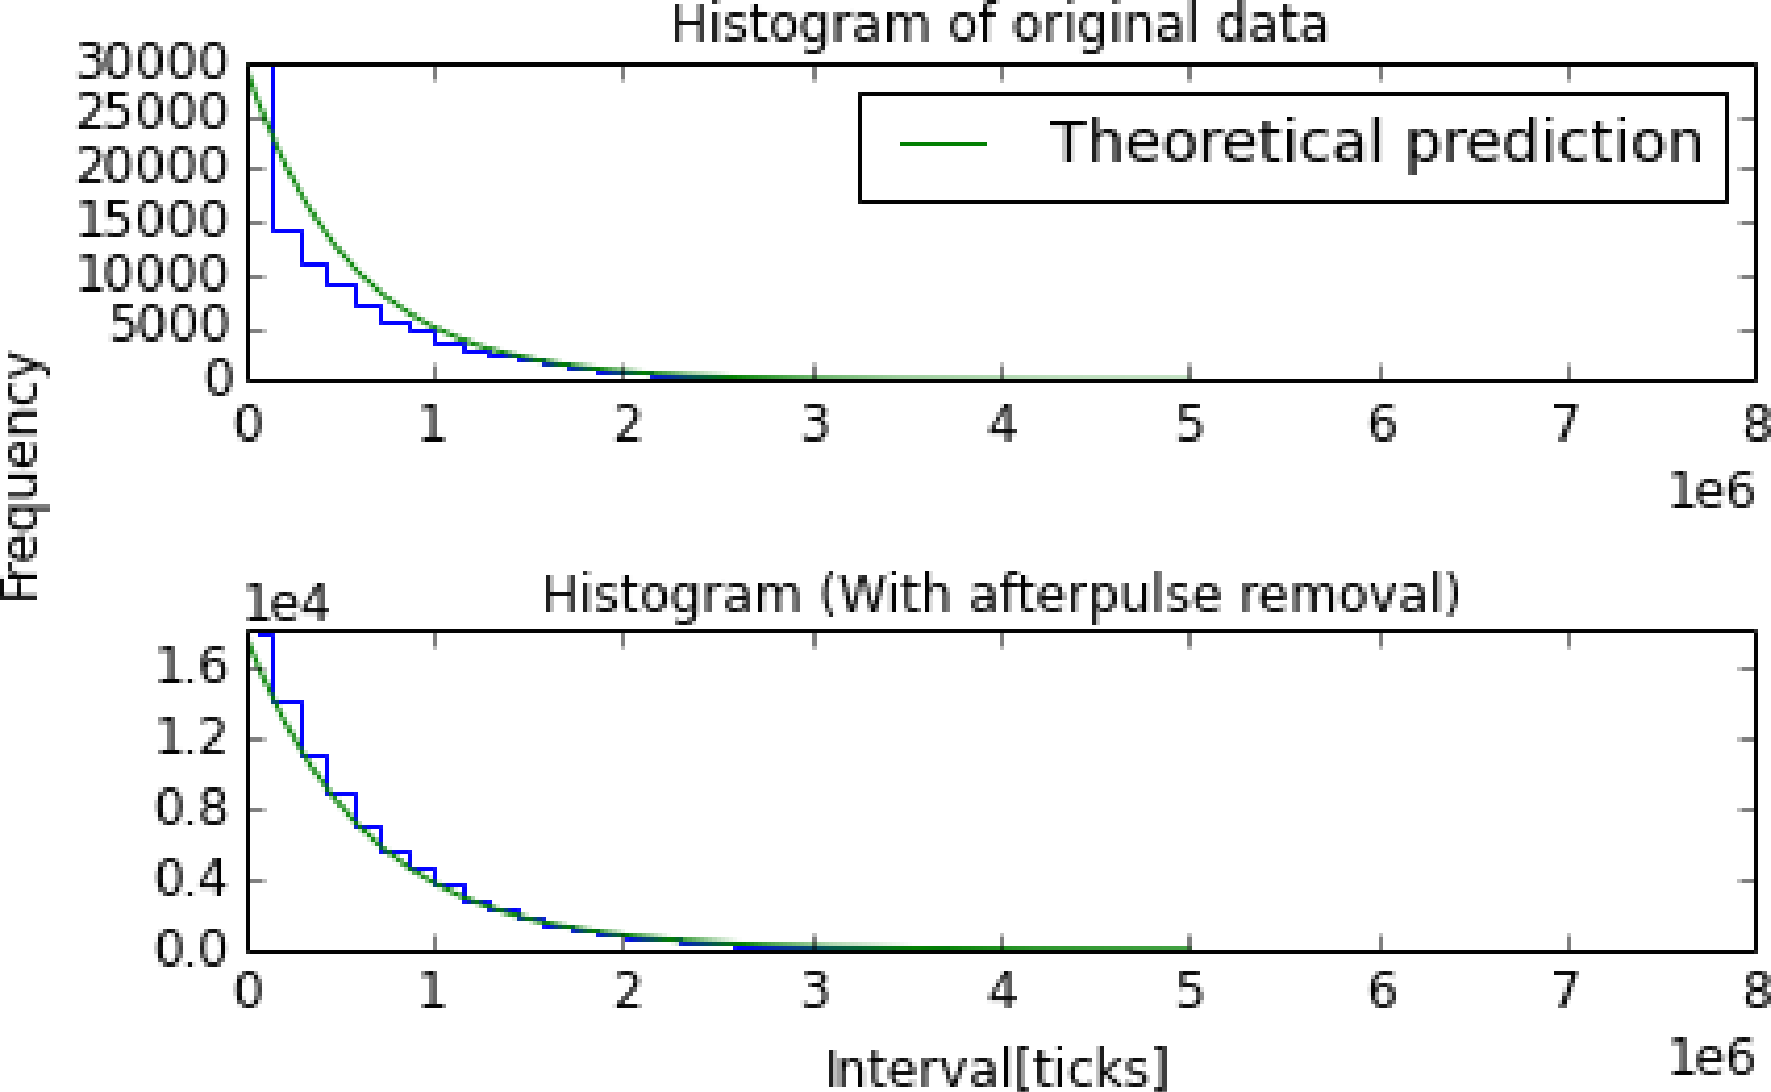
\includegraphics[width=0.5\textwidth]{figures/histogram}
		\caption{Histogram of bin size = 50 before and after gating afterpulses, with the scaled exponential PDF fit.}
		\label{fitted_histo_gate_or_no}
	\end{figure}
 	\subsection{Poisson Distribution}
 	Although closely-related, the Poisson distribution is unlike the exponential distribution in that it is a discrete probability distribution that arises from measuring the number of events that occur within a fixed sampling interval. Both underlying process applies to rare event for very large N, but the experiment method is different. In this case, the experiment is the same, but we change the way the data is represented, as binned data for a fixed time interval.
 	 	\begin{figure}[h]
			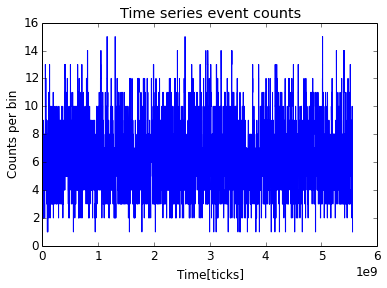
\includegraphics[width=0.5\textwidth]{figures/time_series}
			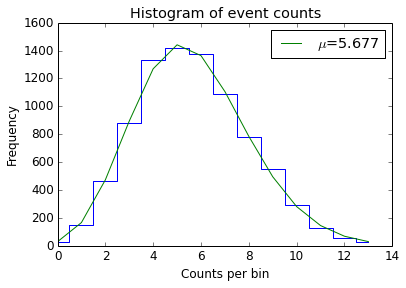
\includegraphics[width=0.5\textwidth]{figures/poisson_histo}
			\caption{The bin counts are obtained by counting the number of photon arrival events that lie within an interval of 3.09 milliseconds. From the time series plot, we see that most time intervals counted 4 to 8 events. This is confirmed by using a Poisson curve fit on the histogram where the value of the fitting parameter is 5.677.}
			\label{poisson}
		\end{figure}
\section{Conclusion\label{end}}
Our findings can be summarized to the following points: 
\begin{itemize}
\item 
\item Since photon arrival is rare and random in the limit of large N , it can be closely follow a Poisson distribution.
\item 
\end{itemize}
In this experiment, we only attempt to mitigate the effect of one type of systematic error vetoing the afterpulses. One possible extensions to this project may be to investigate the effect of other types of systematic error such as dark counts and thermal noise on the quality of the data. This effect can be quantified by measuring the signal to noise ratio and comparisons among different types of PMT.
\end{document}
